%====================================================================================================
% ?????
%====================================================================================================
% TCC
%----------------------------------------------------------------------------------------------------
% Autor				: Jasane Schio
% Orientador		: Gedson Faria
% Co-Orientador		: Angelo Darcy
% Instituição 		: UFMS - Universidade Federal do Mato Grosso do Sul
% Departamento		: CPCX - Sistema de Informação
%----------------------------------------------------------------------------------------------------
% Data de criação	: 01 de Outubro de 2015
%====================================================================================================
% Define o caminho das figuras
\graphicspath{{figuras/}}
\chapter{Fundamentação Teórica} \label{Cap:Fundamentacao}

%\section{Estado da Arte} \label{Sec:EstadoDaArte}
%Como estado da arte foram relacionados os métodos de detecção de objetos em imagens em tempo real e estáticas.

\section{Processamento de Imagens}
\subsection{Detecção de Objetos}
\label{Sec:TiposDeDeteccaoDeObjetos}
%Antes de descrever os métodos de classificação devemos fazer algumas definições:
%\begin{itemize}
%	\item	Em cada detecção de objetos são obtidas as informações sobre a imagem, essas são de acordo com o tipo de detecção desejada. Os dados podem conter informações como posição, tamanho, borda, transformação linear, rotação entre outros. Cada detecção em uma imagem é chamada de pose.
	
%	\item	Métodos de detecção de objeto baseado em classes constroem a classe do objeto baseada em um conjunto de treino. O conjunto de treino é composto por múltiplas imagens exemplo do objeto para que seja assim capturado os aspectos do objeto.
%\end{itemize}

A detecção de objetos pode ser considerada uma técnica herdada do reconhecimento de padrões, da área de aprendizado de máquina, esta consiste em separar objetos por categorias de acordo com uma ou mais características especificas. Quando essa técnica se junta ao processamento de imagens, onde são estas características são acentuadas em um determinado objeto dentro da imagem para assim este se destacar, tornou-se possível a detecção de objetos em imagens, que dentro do campo de visão computacional é uma das áreas que mais obtêm a atenção de pesquisadores. 
O primeiro Framework de métodos que usam base de dados categorizando uma ou mais características de um objetos para fazer o reconhecimento através de aprendizado foi apresentado em 2001 por Viola e Jones\cite{Viola:2001}. Desde o framework de Viola e Jones até os dias atuais muitos métodos e teorias para detecção já foram propostos e implementados, como detecção de faces utilizando um classificador de redes neurais na intensidade de padrões de uma imagem, support vector machine para localizar rostos humanos e carros\cite{Nascimento:2007}, análise de componentes principais, análise independente de componentes, fatoração de matriz não-negativa, análise discriminativa linear, boosting\cite{Roth:2008}, além da classificação binaria, onde se considera a detecção do objeto em tamanho fixo apenas variando na posição na imagem\cite{AmitFelzenszwalb:2014}. 

%Em 2005 Ulusoy e Bishop\cite{Ulusoy:2005} mostraram o quão útil seria categorizar os métodos de detecção de imagens, e os dividiram em duas principais categorias: generativa e discriminativa. Categorias que foram aceitas e utilizadas como mostram Amit e Falzenszwalb\cite{AmitFelzenszwalb:2014} e Roth e Winter\cite{Roth:2008}.

%O método generativo pode ser descrito como um modelo probabilístico para a variância da pose de um objeto juntando com o modelo de aparência, ou seja, um modelo de probabilidade para a aparência da imagem condicional em uma determinada pose, juntamento com um modelo de fundo. Os parâmetros do modelo são estimados a partir de dados retirados de treinamento e as decisões são baseadas nas probabilidades anteriores\cite{AmitFelzenszwalb:2014}. Em resumo o método generativo tenta encontrar uma representação adequada dos dados originais através da aproximação dos dados originais, mas mantendo o máximo de informação possível\cite{Roth:2008}.

%Já o modelo discriminativo tipicamente constrói um classificador que pode discriminar entre imagens (ou sub-imagens) contendo o objeto e as que não contém o objeto. Os parâmetros do classificador são selecionados para minimizar os erros nos dados de treino\cite{AmitFelzenszwalb:2014}.


%	Ulusoy\cite{Ulusoy:2005} apontou as principais vantagens dos dois metodos. 
%Segundo Ulusoy e Bishop\cite{Ulusoy:2005} o método generativo se destaca por tratar perda de dados ou dados parcialmente rotulados, pela facilidade em que uma nova classe pode ser incrementada na classificação condicional de densidade, independentemente das classes anteriores, e por conseguir facilmente lidar com composição de objetos (ex: óculos, chapéus...), considerando que os modelos discriminativos precisar analisar todas as combinações durante o treinamento. Amit e Felzenszwalb\cite{AmitFelzenszwalb:2014} ainda aponta que as vantagens descritas sobre o método discriminativo são ditas como a flexibilidade do modelo  que pode ser utilizado em regiões do espaço de entrada onde as probabilidades posteriores diferem significativamente de 0 ou 1, ao passo que as abordagens detalhes generativas modelo de distribuição de X, que podem ser irrelevantes para determinar as probabilidades posteriores, além de ser tipicamente muito rápido em fazer previsões para os novos pontos (teste) de dados, enquanto os modelos generativos muitas vezes exigem solução iterativa, e pela igualdade de circunstâncias, seria de esperar que os métodos discriminativos tenham melhor desempenho preditivo, uma vez que são treinados para prever o rótulo de classe em vez de a distribuição conjunta de vetores e alvos de entrada.

\subsection{Detecção de Bordas}
Para um objeto poder ser detectado por algum método de detecção a imagem passa por um processo de segmentação. A segmentação pode ser dita como o processo de divisão da imagem em objetos\cite{Gonzalez:2008}. De acordo com Wangenheim\cite{Wangenheim:2014} o processo de segmentação se baseia em dois conceitos: similaridade e descontinuidade. A descontinuidade é o processo onde se separa o fundo das partículas e estas umas das outras, através de linhas, bordas ou pontos. Já a similaridade é o processo onde os pixeis provenientes da descontinuidade são agrupados de acordo com a proximidade um dos outros para formar os objetos de interesse. De acordo com Canny\cite{Canny:1986} o processo de detecção de bordas é um processo simplificado que serve para diminuir drasticamente o total de dados a serem processados e ao mesmo que o mesmo preserva informações valiosas sobre os objetos, este tambem é considerado um processamento de imagem de baixo nivel, uma vez que age diretamente na imagem original apenas melhorando-a. É muito comum a ocorrência de ruídos quando se trata da detecção de bordas, e por sua vez para evitar esses ruídos é necessário a suavização da imagem antes de fazer a detecção. Vale\cite{Vale:2002} lembra que a suavização possui pontos negativos como perda de informação e deslocamento de estruturas de feições proeminentes no plano da imagem. Além disso, existem diferenças entre as propriedades dos operadores diferenciais comumente utilizados, o que ocasiona  bordas diferentes.Assim, como dito por Ziou e Tabbone citados por Vale\cite{Vale:2002}, se torna difícil encontrar um algoritmo que tenha bom desempenho em diferenciados contextos e capture os requisitos necessários aos estágios subsequentes do processamento. 
Quando se trata de detecção de bordas existem dois critérios\cite{Canny:1986} para essa detecção que devem ser levados em consideração, Taxa de Erro e Localização\cite{Vale:2002}. 
\begin{description}
	\item[Taxa de Erro] É importante que as bordam contidas na imagem não sejam confundidas ou perdidas e ainda que não sejam detectadas bordas falsas. É necessário que o algoritmo de detecção de borda tenha uma baixa taxa de erro para que seja eficiente\cite{Wangenheim:2014, Canny:1986, Vale:2002}.
	\item[Localização] A distância entre os pixels de borda encontradas pelo algoritmo e a borda atual deveriam ser o menor possível\cite{Wangenheim:2014}.
\end{description}
Ao tentar aplicas esses dois critérios para desenvolver um modelo matemático para detecção de bordas sem a necessidade de base em regras preestabelecidas em seu artigo,
\textit{A Computational Approach to Edge Detection}, Canny percebeu que somente esses dois critérios não eram o suficiente para obter uma boa precisão da detecção de bordas. E então propôs um terceiro critério: Resposta.
\begin{description}
	\item[Resposta] Para contornar a possibilidade de mais de uma resposta para a mesma borda, ou seja o detector de bordas não deveria identificar múltiplos pixels de borda onde somente exista um único pixel\cite{Wangenheim:2014, Canny:1986, Vale:2002}.
\end{description}


Com o acréscimo do terceiro critério então nota-se que o processo de detecção de bordas de Canny
mostrou-se bastante flexível, independente da origem da imagem utilizada\cite{Vale:2002}.
 \begin{figure}[!h]
	\centering
	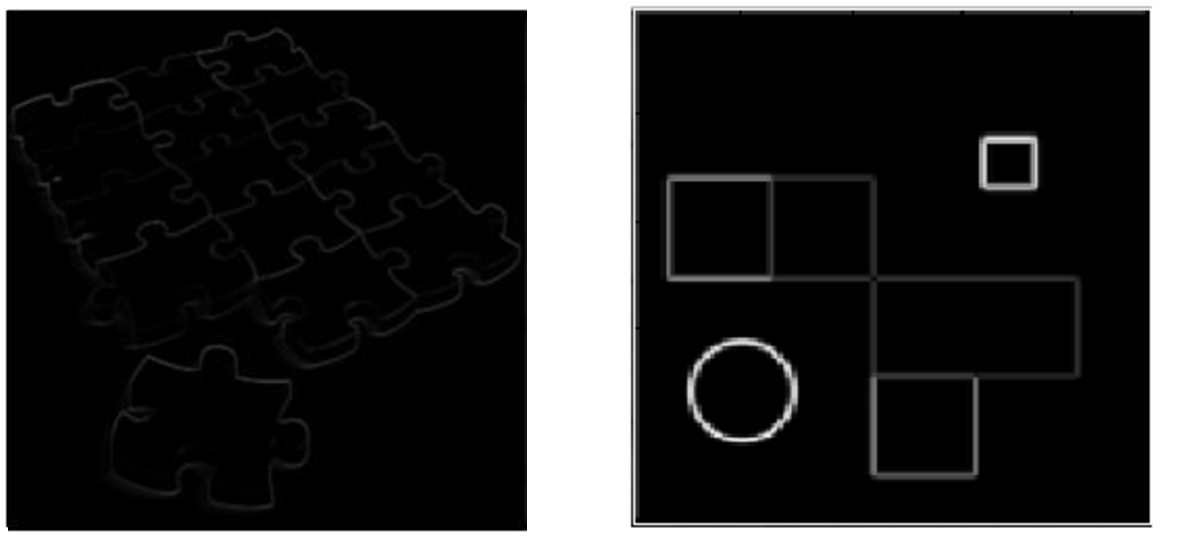
\includegraphics[width=0.8\textwidth]{canny.pdf}
	\caption{Detecçcao de Borda com Algoritmo de Canny\cite{Saini:2013} }
	\label{Canny}
\end{figure}







\section{Cores} \label{Sec:Cores}


O olho humano é capaz de identificar cores mesmo com as mais diferentes interferências, luminosidade, tonalidade, intensidade, entre outras ações de agentes externos graças aos \textbf{cones} e \textbf{bastonetes}. Os bastonetes são os responsaveis por distinguirem tons de cinza e pela visão periferica e tem como caracteristica serem sensiveis a baixo nivel de luminosidade\cite{Azevedo:2003}, os cones, por sua vez, são sensiveis ao alto nivel de iluminação e responsaveis pela percepçao de cores\cite{Azevedo:2003}. Segundo a teoria tricomática de Thomas Young e mais tarde estudada por Hermann von Helmholtz\cite{Azevedo:2003}, a retina humana é formada por três tipos de fotopigmentos que seriam os três receptores de cor, ou seja respondiam ao comprimento de onda de apensa três cores: Vermelho, Verde e Azul. A informação obtida através do sistema visual humano é assimilada pelo cérebro humano e ligando a cor a sua aparência levando em consideração o aprendizado que obtivemos sobre a mesma, já para uma máquina cores são números, códigos, cada cor contém um código especifico e cada uma de suas variâncias também. Para o nosso cérebro é muito fácil entender, exemplo, que o verde, verde lima, verde escuro são todos verde, apenas com tonalidades diferentes, já para o computador estas são: (0,255,0),(50,205,50),(0,128,0), no padrão de cor RGB. Mas se for aplicado luminosidade nessas cores, por exemplo, elas ainda se tornam outras diferentes cores, um código diferente para cada luminosidade possível.




Para poder explicar as propriedades e comportamentos das cores em determinadas circunstâncias, surgiram os \textbf{Sistemas de cores}. Devido a complexidade existente em explicar todos os aspectos relacionados às cores são utilizados diversos sistemas para descrever as mais diferentes caracteristicas das cores e sua percepção pelo ser humano\cite{Azevedo:2003}.  Dentro os sistemas mais conhecidos, estão o RGB, HSV E HSL, sistemas quais serão neste trabalho.

Segundo Azevedo\cite{Azevedo:2003} o universo de cores que podem ser reproduzidas por um sistem é chamado de \textbf{Espaço de Cores}. De acordo com Foley et. al citado por Souto\cite{Souto:2003} espaço de cores é um sistema tridimensional de coordenadas, onde cada eixo refere-se a uma cor primária. A quantidade de cor primária
necessária para reproduzir uma determinada cor, é atribuída a um valor sobre o eixo
correspondente. O espaço de cores pode ser entendido como a quantidade de detalhamento, tonalidades de uma cor, dentro do espectro de cores de um determinado modelo de cor.

 \begin{figure}[!h]
	\centering
	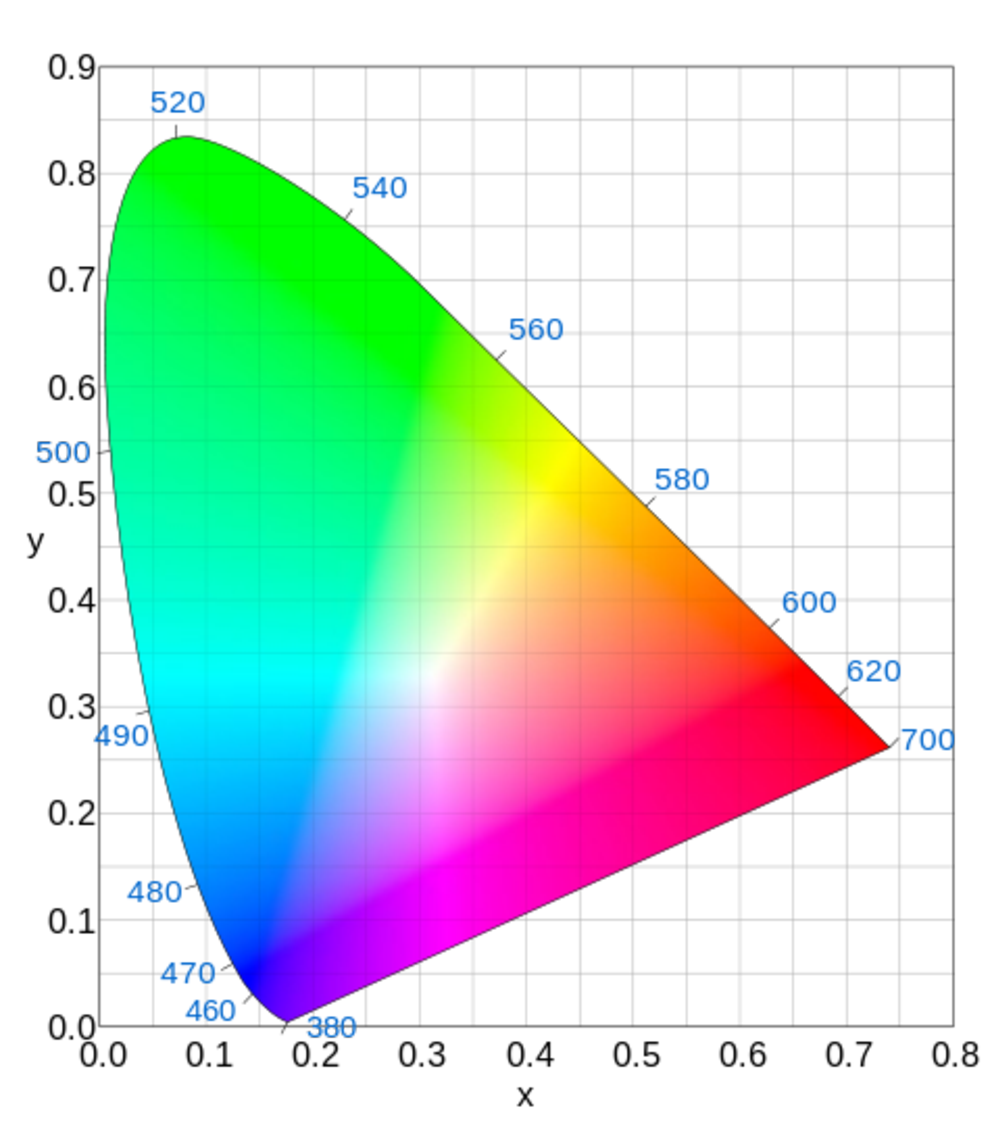
\includegraphics[width=0.25\textwidth]{graficocie.pdf}
	\caption{Universo de cores estabelecido pelo CIE.}
	\label{EspacodeCores}
\end{figure}


Quando fez sua primeira experiência com a decomposição da luz em um prisma para obter cores Newton percebeu que não havia a cor branca. Ele tentou então misturar as sete cores que obteve para gerar a branca, sem sucesso. 
 Para conseguir cobrir todas as alterações e caracteristicas as cores em 1921 a Comissão Internacional de Iluminação (CEI)\cite{Souto:2003} definiu três primarias(X, Y e Z) que podem ser combinadas para formarem todas as cores e entendeu-se que existe duas formas de se obter cores: através da emissão ou reflexão de luz, espaços RGB e CMY respectivamente, \figurename{ 2.2}. Assim entendeu-se então porque em seu experimento Newton não obteve sucesso para gerar a cor branca, pois parar gerar a cor branca é necessário a soma das três cores primarias azul, verde e vermelho, uma vez que seu experimento utilizava a reflexão e não emissão de cores.
 \begin{figure}[!h]
	\centering
	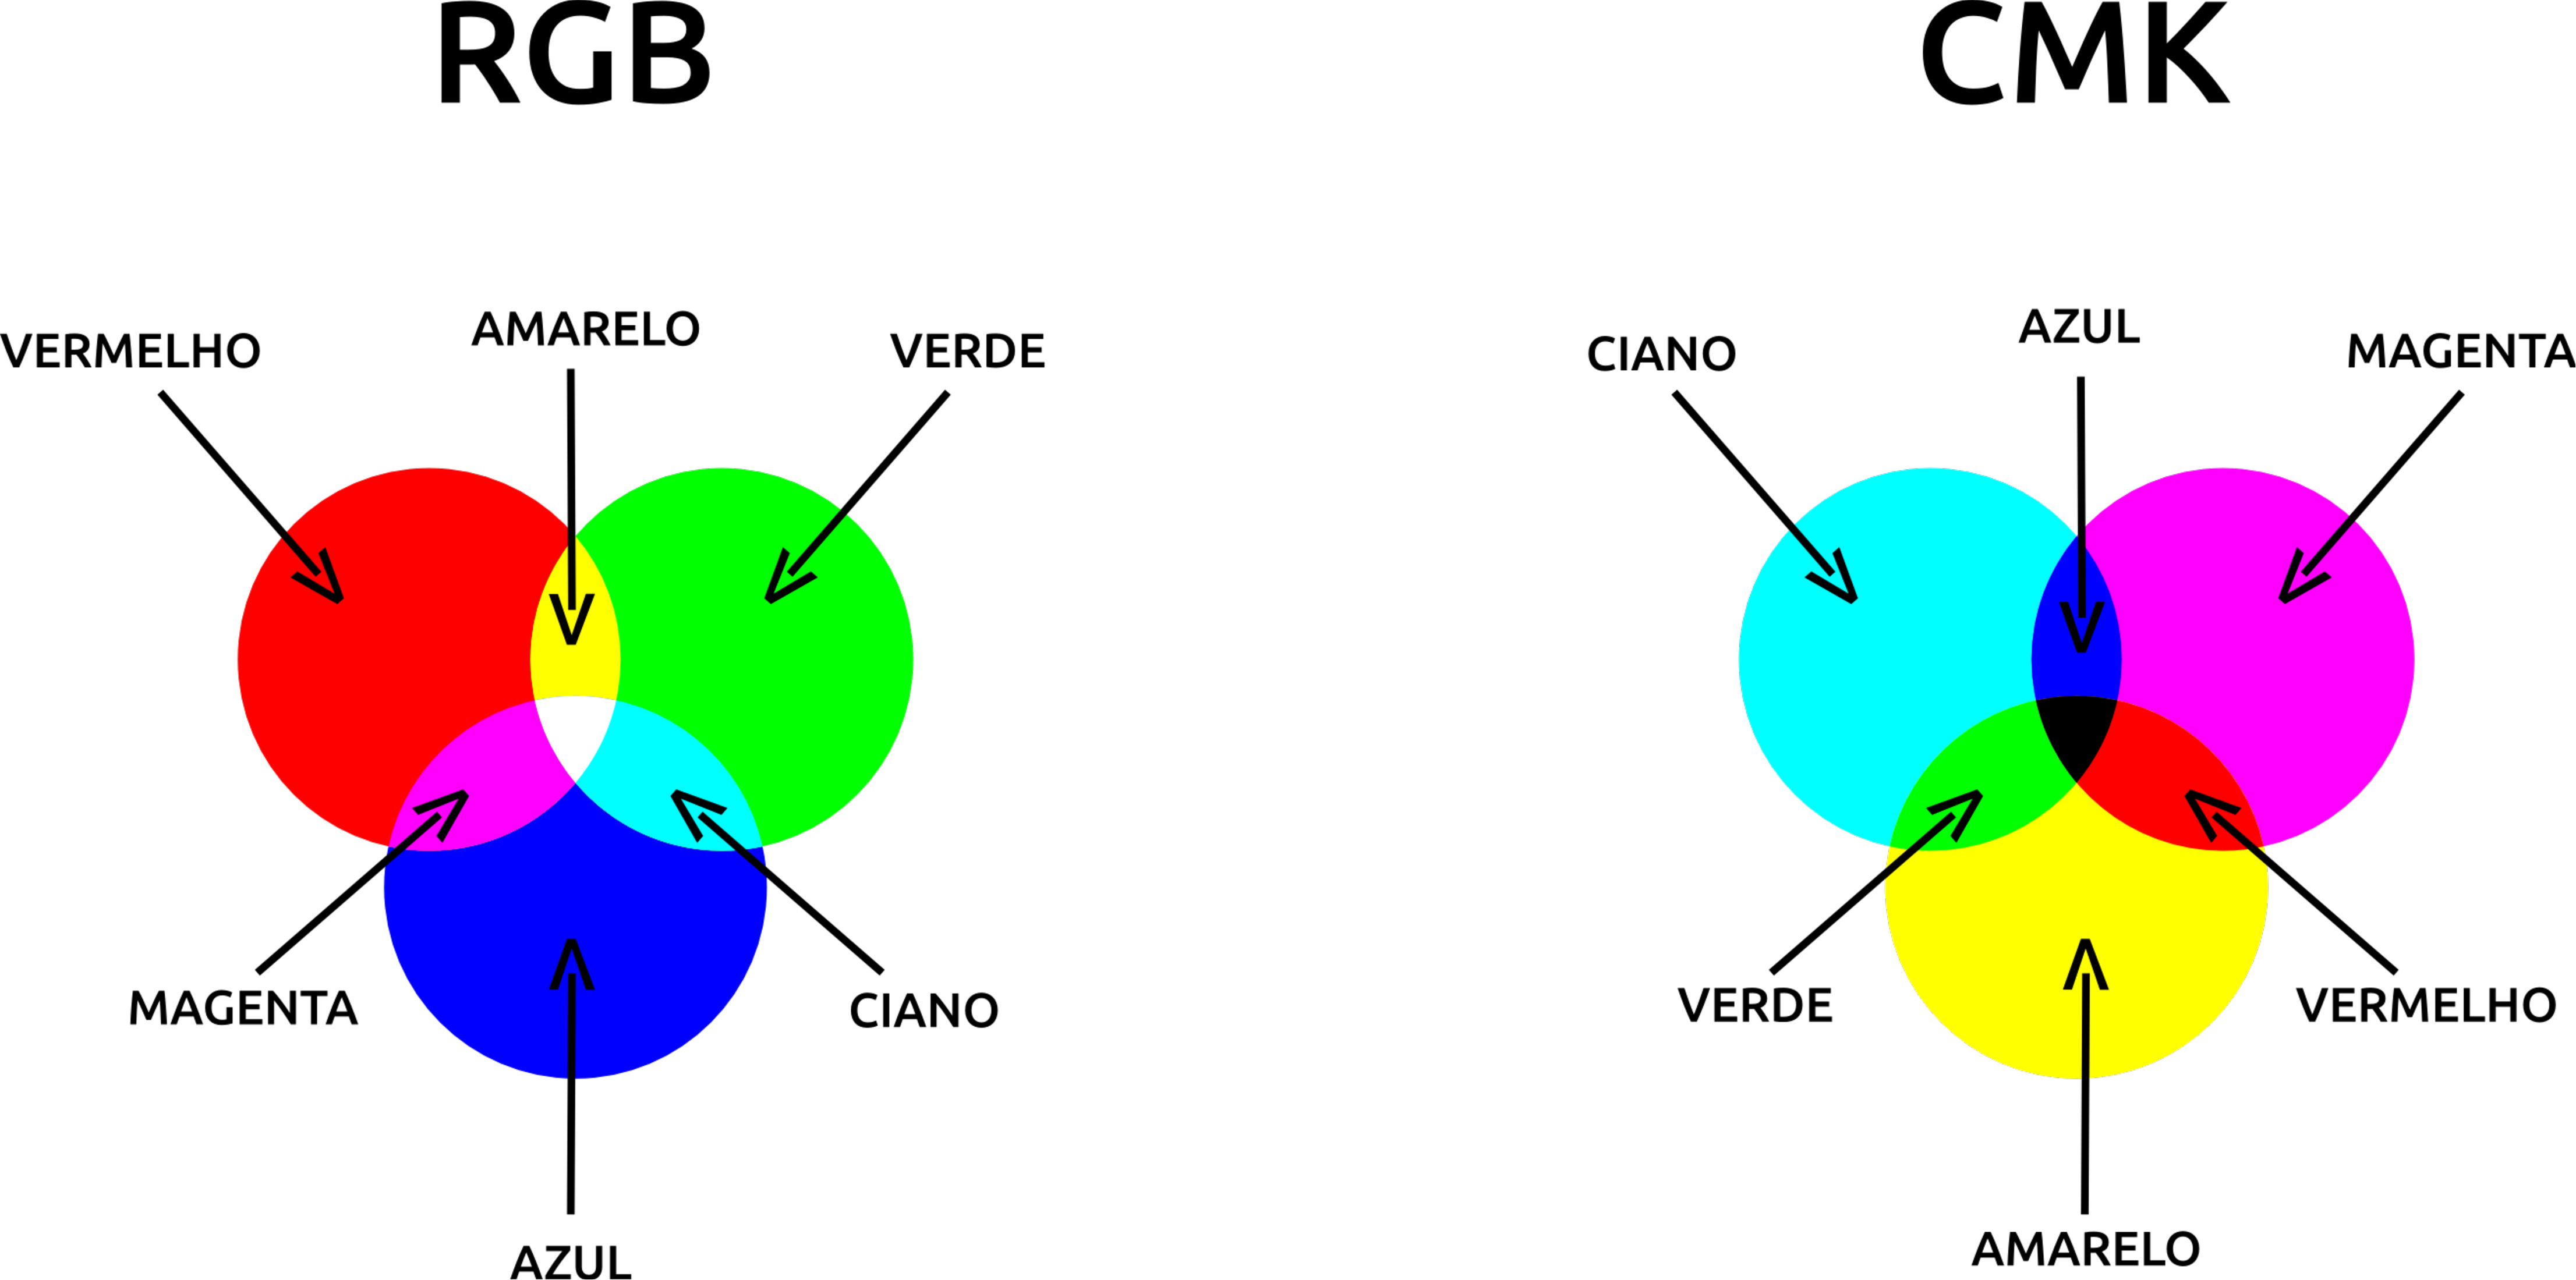
\includegraphics[width=0.5\textwidth]{espacos.pdf}
	\caption{Exemplo dos espaços de cores RGB E CMY.}
	\label{EspacodeCores}
\end{figure}



Para utilização pratica de sistemas e espaços de cores e descreverem as cores foram criados modelos de cores, neste trabalho falaremos sobre o RGB e HSV, pois são os modelos usados durante o desenvolvimento.
Modelo de cores são modelos matemáticos utilizados para classificação das cores de acordo com sua tonalidade, saturação, luminosidade ou crominância na tentativa de conseguir cobrir o maior número de cores possíveis e assim simulando a visão. A representação da cor é definida por um único ponto em um modelo tridimensional. 
Os modelo de cores tem função definir as cores nos programas gráficos de computadores de forma que combine com a 
percepção das cores pelo sistema visual humano e utiliza três eixos similares para definirem a cor\cite{Leao:2005}.

O modelo de cores RGB pode ser considerado mais básico dos modelos de cores. Seu nome possui a mesma definição do espaço de cores RGB. Ele não utiliza de nenhum atributo como luminosidade ou tonalidade, por exemplo, para a definição da cor apenas a adição das cores primarias, azul, verde e vermelho. É este também o padrão mais usado e conhecido. Os valores de R,G e B variam de 0 à 255.


\begin{figure}[!h]
	\centering
	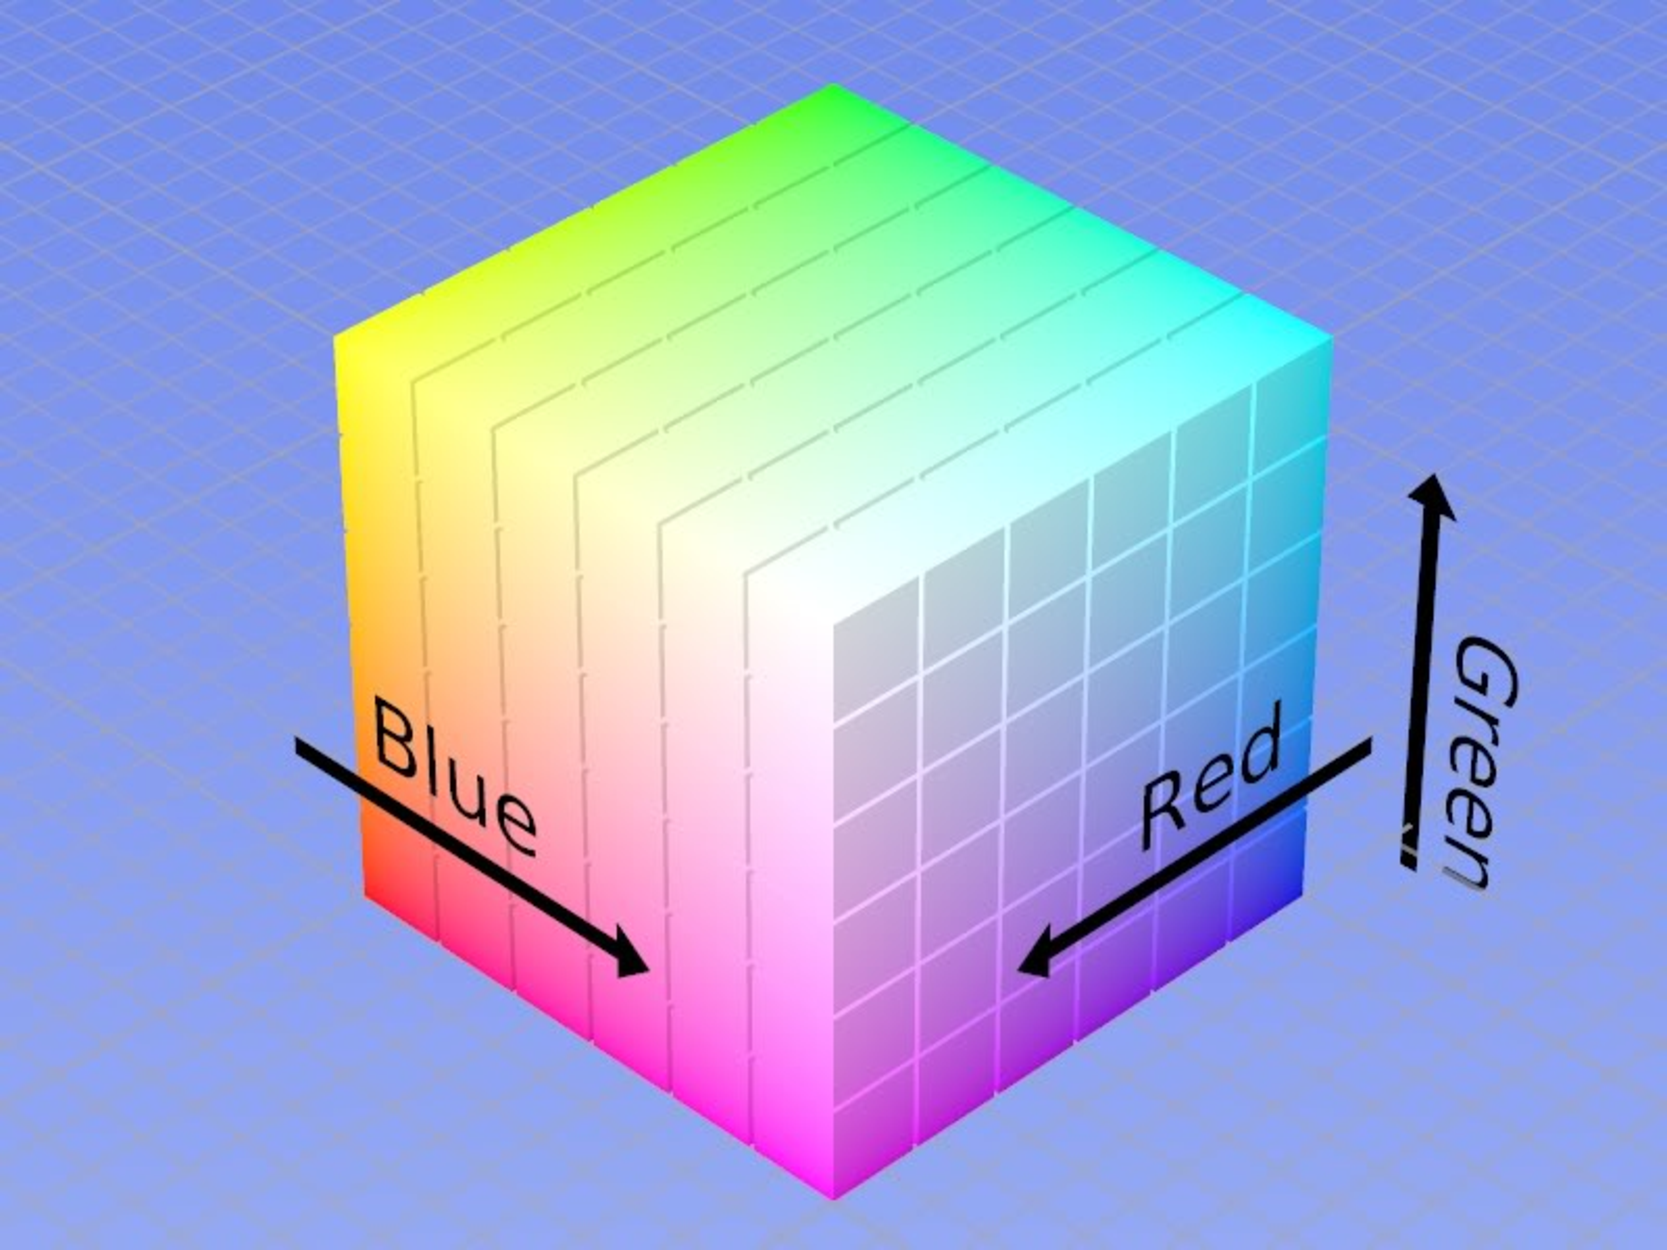
\includegraphics[width=0.4\textwidth]{rgb.pdf}
	
\caption{Exemplo do Modelo de Cor RGB.	 Horvath\cite{ImagensHSLHSVRGB}  }
	\label{ModeloRGB}
\end{figure}



O modelo HSV define tonalidade (hue) que é a cor em si, variando de 0 a 360º, a saturação(saturnation) que define o grau de pureza da cor, variando de 0 a 1, obtido pela mistura da tonalidade com a cor branca e brilho (value) que tenta fazer referência à percepção humana\cite{Leao:2005} que é a intensidade da cor, escala de tons de cinza\cite{Azevedo:2003}, variando também de 0 a 1.


\begin{figure}[!h]
	\centering
	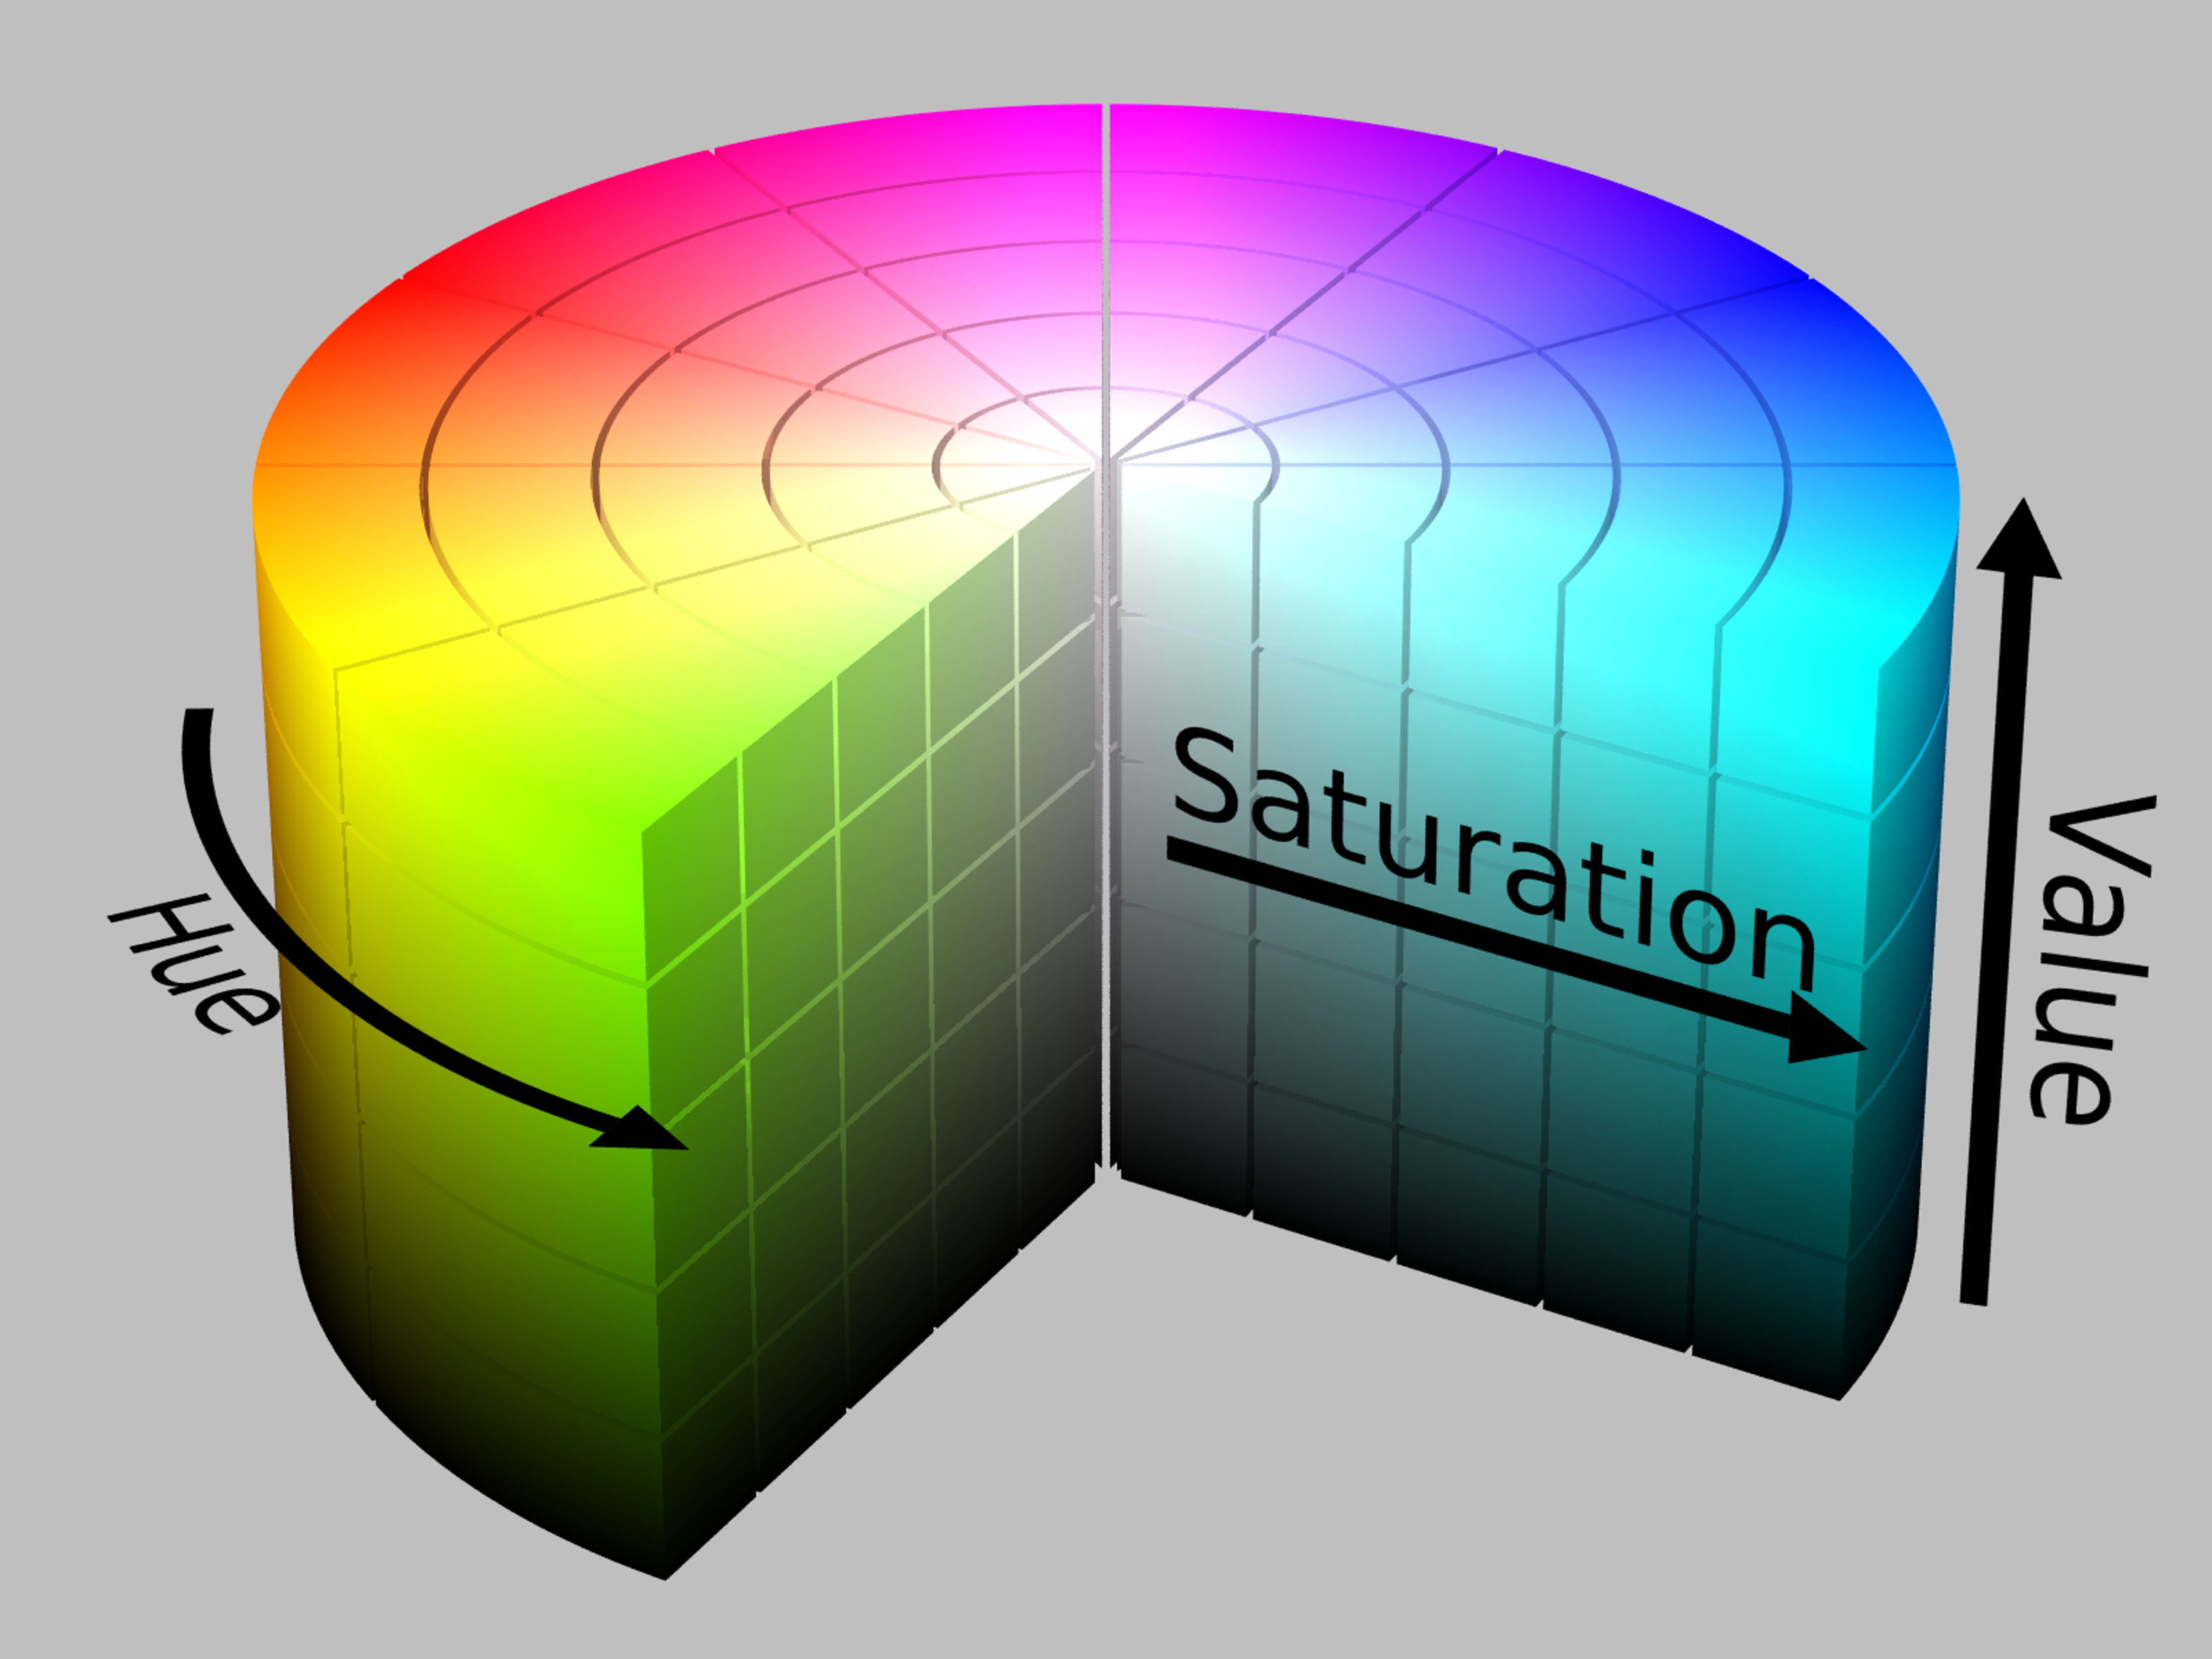
\includegraphics[width=0.4\textwidth]{hsv.pdf}
	
	\caption{Exemplo do Modelo de Cor HSV, Horvath\cite{ImagensHSLHSVRGB}}
	\label{ModeloHSV}
\end{figure} 


O sistema HSV utiliza definições de cor mais intuitivas que o conjunto de cores primarias, por isso são mais adequados quando se necessita obter varias tonalidades.

\section{Futebol de Robôs}
 Visto como um dominio bastente complexo, dinamico e imprevisivel\cite{Costa:2000}, o futebol de robos surgiu como uma tentativa de promover pesquisas nos campos de Inteligencia Artificial e robotica, pela avaliacao teorias, algoritmos e arquiteturas atraves problemas padrao\cite{Kitano:1997}.
 A Equipe Cedro se enquadra na categoria IEEE Very Small Size. Esta categoria é regulamentada pelo Instituto de Engenheiros Eletricistas e Eletrônicos (IEEE) e possui regras baseadas na MiroSot\cite{Rosa:2015}. O futebol de robôs se assemelha ao futebol humano onde o objetivo do jogo é fazer gols para vencer a partida, porem tendo regras adaptadas para o "âmbito" robótico. 
 Rosa\cite{Rosa:2015} em seu trabalho de graduação faz uma boa enumeração das regras básicas:
 \begin{itemize}
 \item A partida dura 10 minutos com dois tempos de 5 minutos;
  \item Há um intervalo de 10 minutos entre um tempo e outro;
   \item Cada time tem direito a dois tempos de 2 minutos que podem ser pedidos a qualquer
   momento;
    \item Caso a diferença de gols entre os dois times chegue a 10 a partida é encerrada;
     \item Uma falta ocorre quando há mais de um robô de um mesmo time dentro de sua própria
     área de gol ou quando um robô empurrar outro robô de outro time;
     \item Um pênalti ocorre quando a bola fica mais de 10 segundos dentro de alguma das áreas;
     \item Um chute-livre ocorre quando os robôs ficam travados por mais de 10 segundos, caso
     ocorra, o juiz posiciona a bola na marca de chute-livre mais próxima de onde ela ficou
     parada e posiciona os robôs de cada time equidistantes a bola;
     \item A cada inicio de partida ou gol feito a bola deve ser posicionada no centro do campo e os
     robôs devem ser posicionados de acordo com a posse de bola.
 \end{itemize}
